%!TEX root = dolgozat.tex
%%%%%%%%%%%%%%%%%%%%%%%%%%%%%%%%%%%%%%%%%%%%%%%%%%%%%%%%%%%%%%%%%%%%%%%
\chapter{Implementation}\label{ch:IMPLEMENTATION}

\begin{summary}
	In this chapter E-me is described from a technological standpoint.
\end{summary}

%%%%%%%%%%%%%%%%%%%%%%%%%%%%%%%%%%%%%%%%%%%%%%%%%%%%%%%%%%%%%%%%%%%%%%%
\section{Technologies}
Here I list the technologies used for building the application with logos, descriptions for each, 6-7 pages.

\begin{itemize}
	\item Backend
	\begin{itemize}
		\item .NET 5
		\item Entity Framework Core 5
		\begin{itemize}
			\item Code-first
			\item Microsoft SQL Server
			\item additional Data Encryption layer
		\end{itemize}
		\item NSwag
		\item Serilog
		\item AutoMapper
		\item Newtonsoft Json
		\item Windows CNG (Cryptographic Next Generation) API
	\end{itemize}
	\item Frontend
	\begin{itemize}
		\item Xamarin Forms
		\item Telerik UI for Xamarin
		\item Telerik Document Processing Core
		\item Syncfusion Xamarin PDF viewer
		\item GoogleVision API - BarcodeScanner XF implementation
	\end{itemize}
\end{itemize}

\section{Architecture}

E-me follows a commonly used N-tier architecture with three main parts: data, application (backend) and presentation (frontend) layers.
Each of these tiers can be broken down into layers that are defined by their responsibilities within the application.
This tier-based architectural approach adds modularity to the application which results in a low cost of change when compared to a single-tier structure.


\begin{figure}[H]
	\centering
	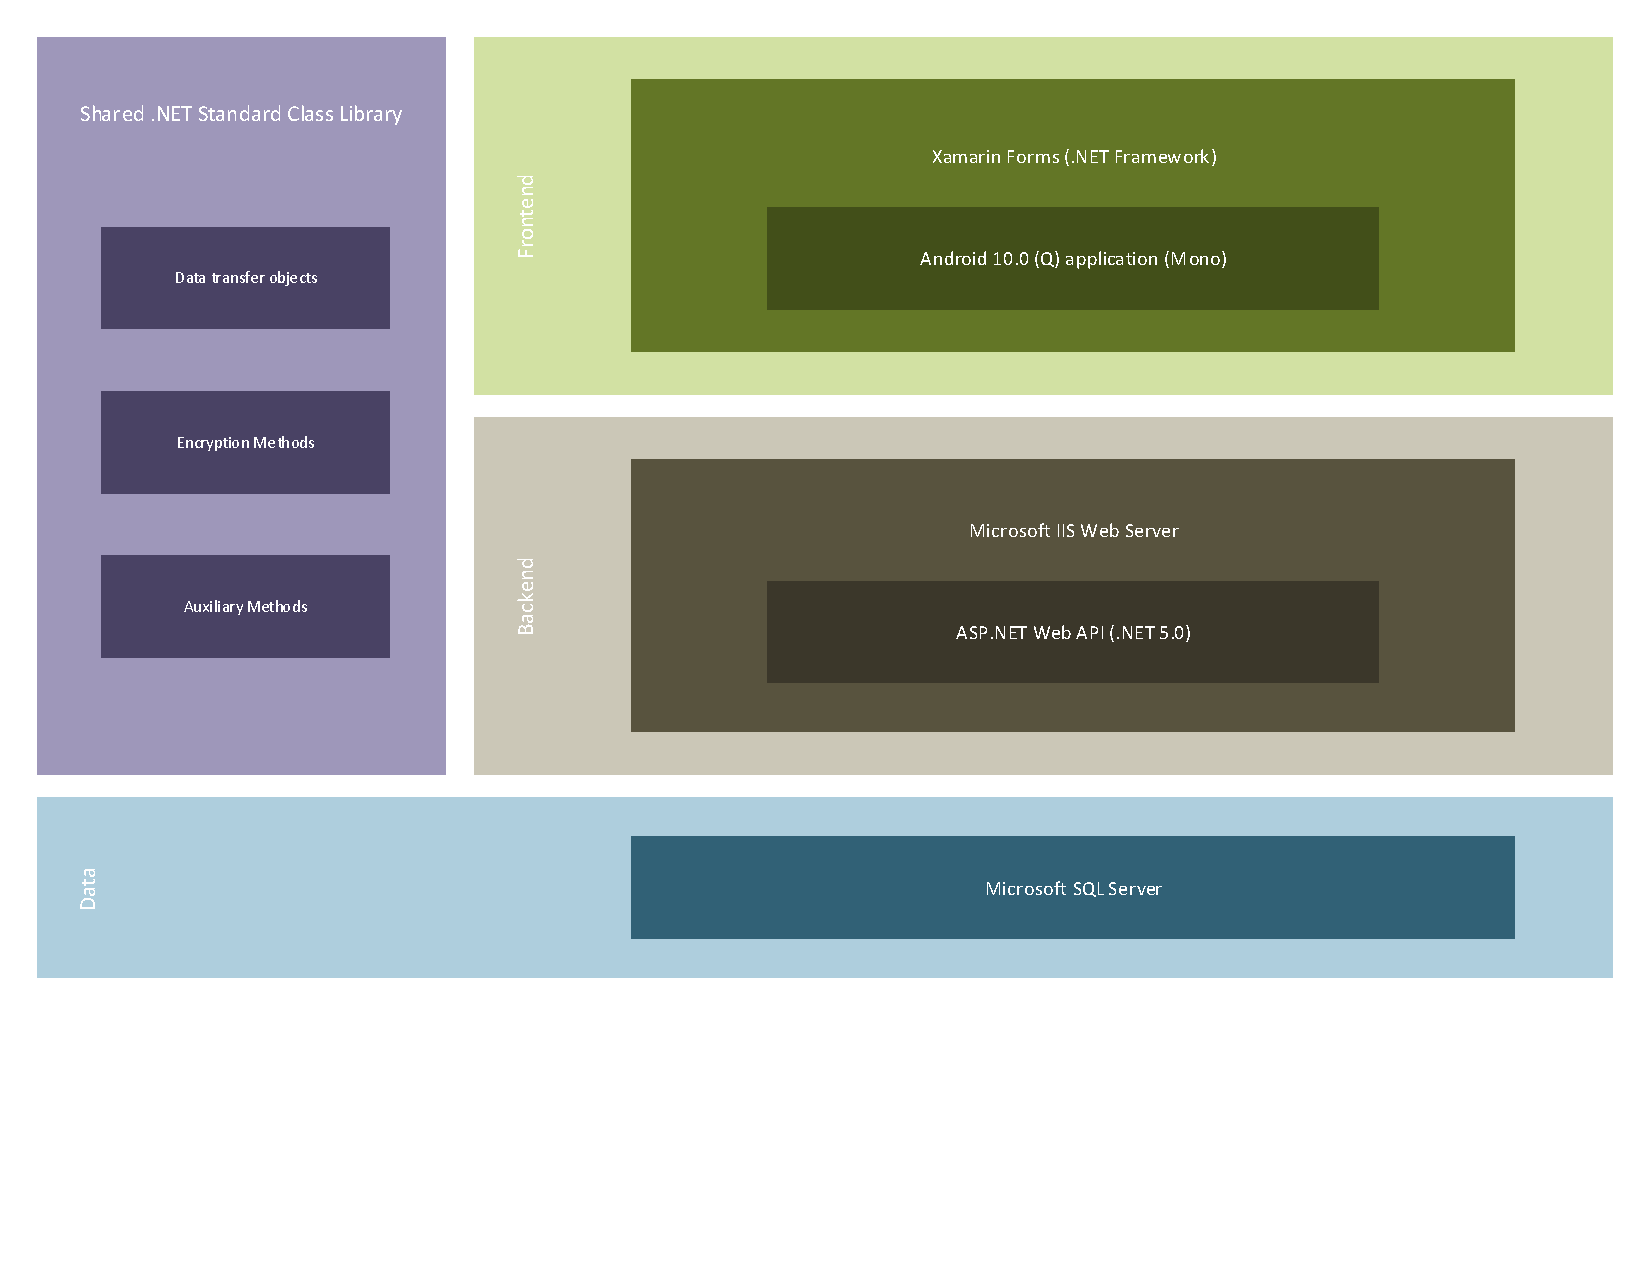
\includegraphics[scale=0.57]{general-architecture}
	\caption{General architecture}
\end{figure}

Along with the low cost of change, the independence of the layers allows for future expansion of 
the application by means of multiple frontend platforms (ex. web applications, desktop applications), cloud storage/services and additional
Web API's that can easily be integrated into the existing application.
This, combined with the high compatibility of the .NET 5.0, provides a high level of scalability and maintainability for the application.

\subsection{Application/Backend layer}

The architecture of the application layer has a similar design approach to the general architecture.
Consisting of 4 layers, the backend of the application follows the single-responsibility principle in it's core.
Because of it's vertical structure, each layer is dependent on one single layer that is directly below it, providing a high level
of maintainability.

\begin{figure}[H]
	\centering
	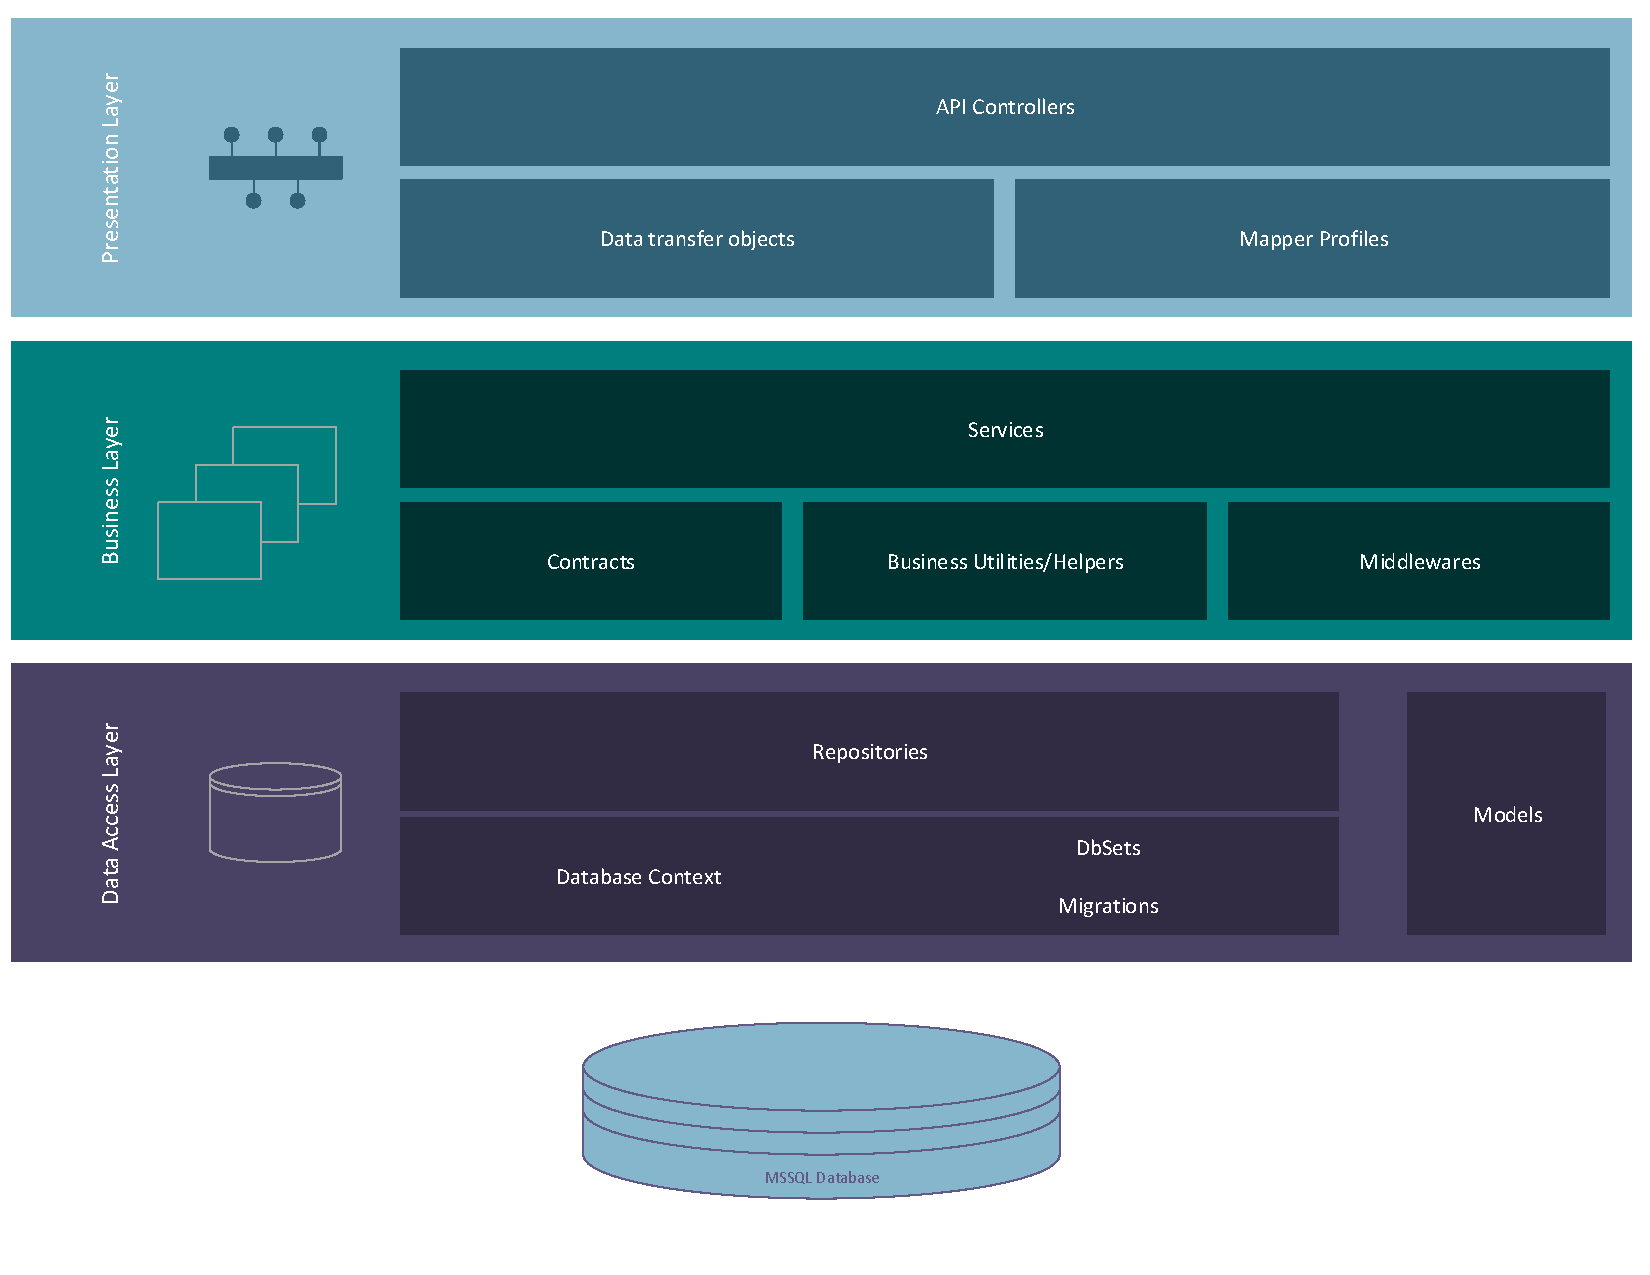
\includegraphics[scale=0.57]{backend-architecture}
	\caption{Backend architecture}
\end{figure}

\begin{figure}[H]
	\centering
	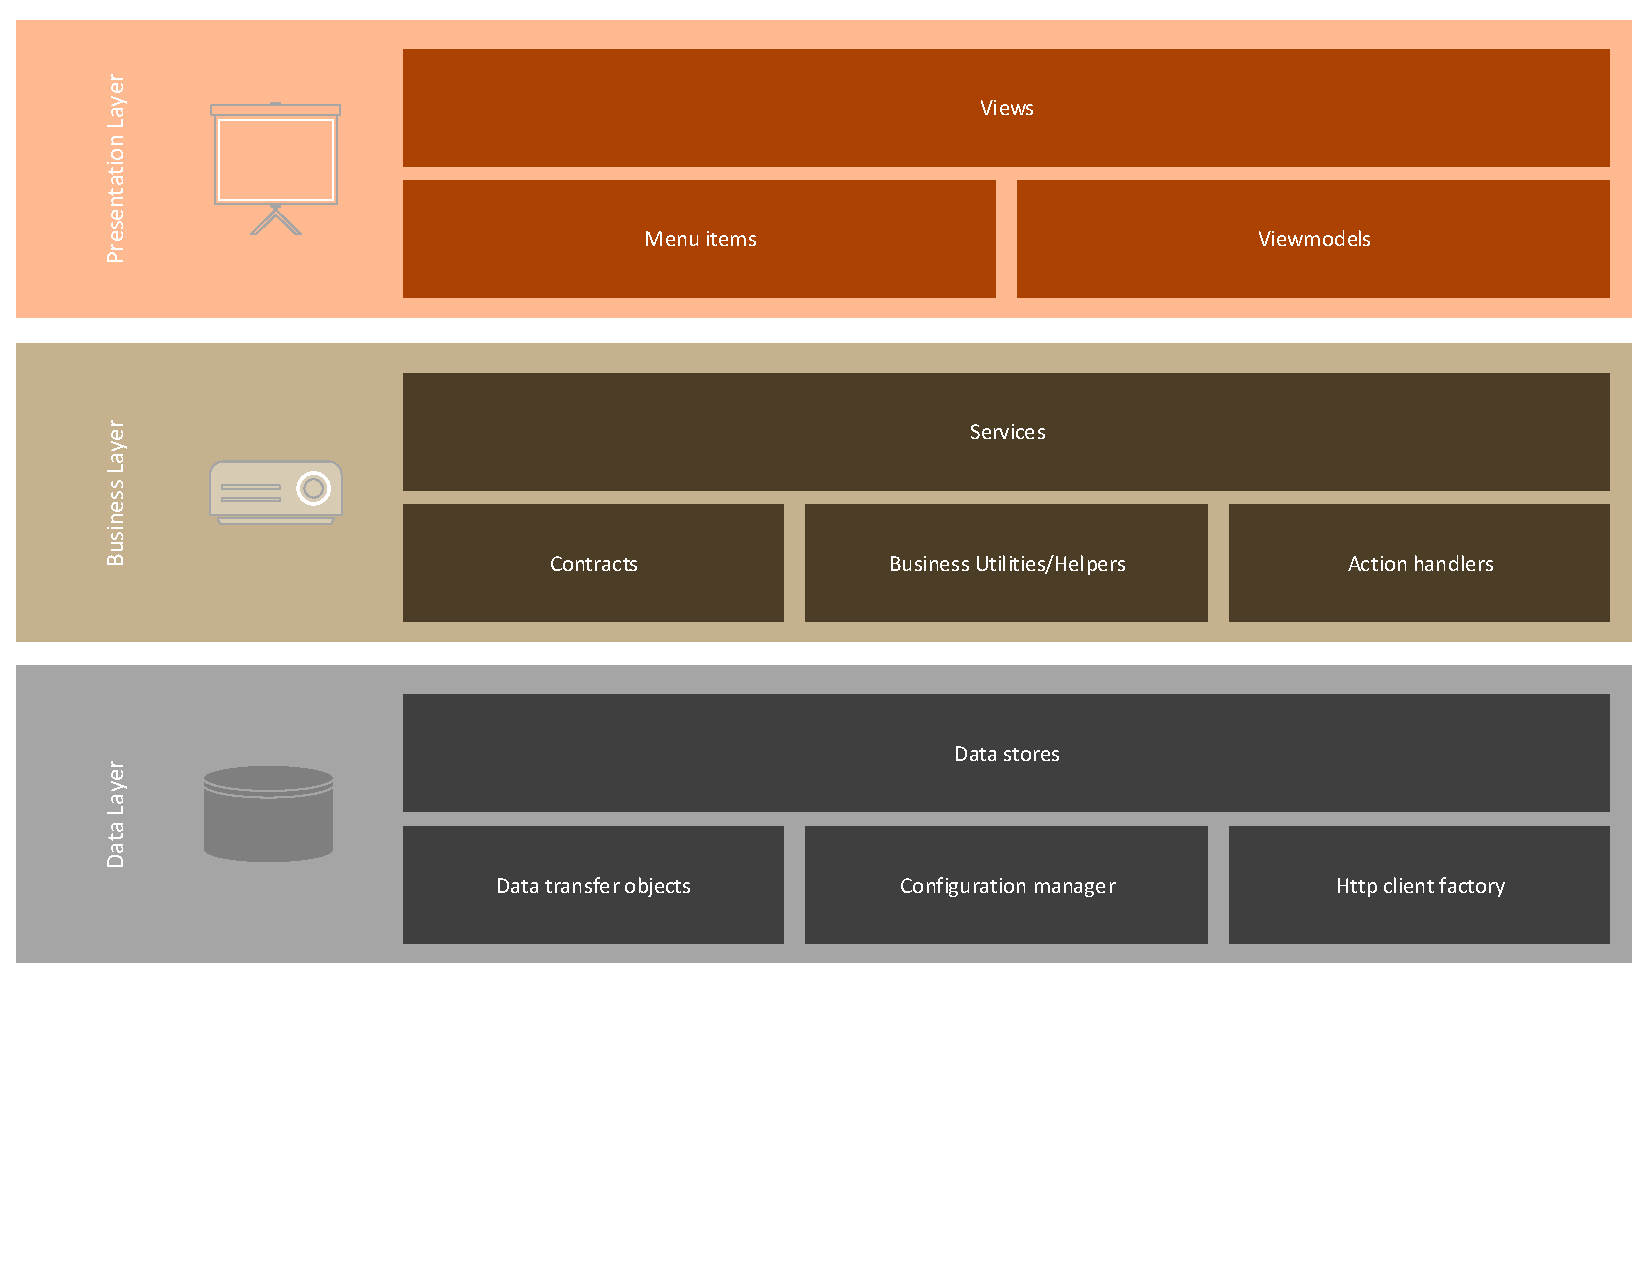
\includegraphics[scale=0.57]{frontend-architecture}
	\caption{Frontend architecture}
\end{figure}

\begin{figure}[H]
	\centering
	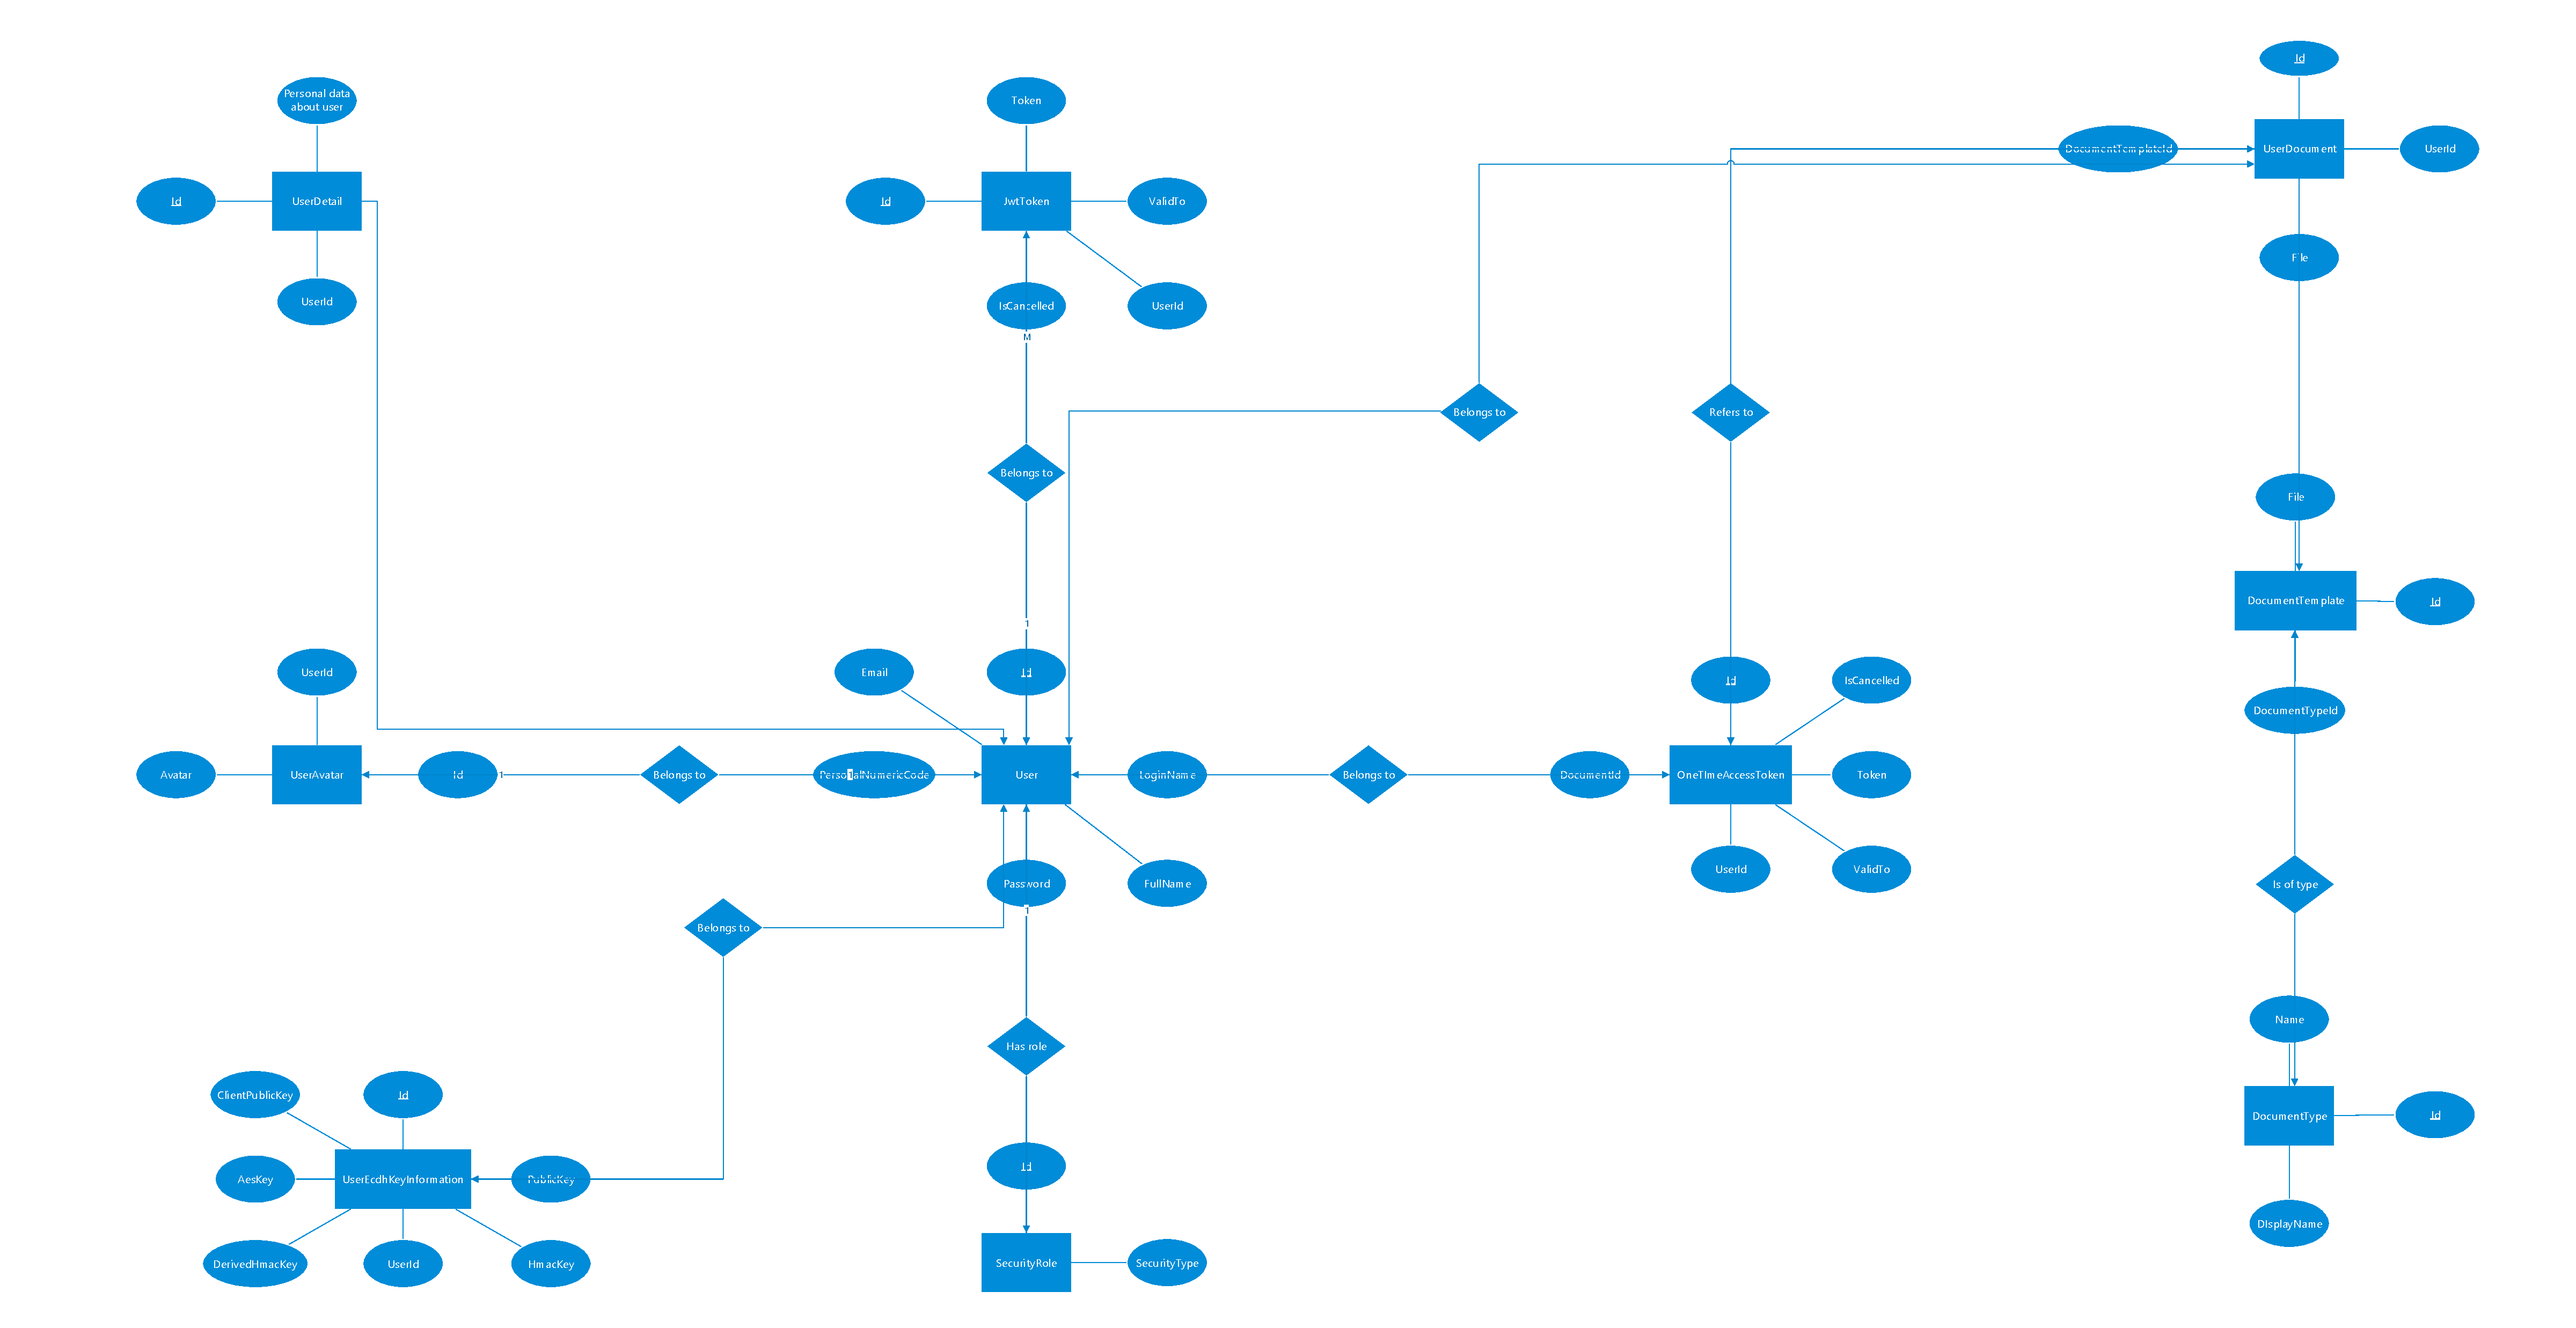
\includegraphics[scale=0.29]{entity-relationship-diagram}
	\caption{Model UML}
\end{figure}


\begin{itemize}
	\item General 3-tier architecture
	\begin{itemize}
		\item diagram
		\item general description
	\end{itemize}
	\item Backend multi-tier architecture
	\begin{itemize}
		\item diagram
		\item general description
	\end{itemize}
	\item Model UML diagram
	\begin{itemize}
		\item diagram
		\item general description
	\end{itemize}
	\item Frontend multi-tier architecture
	\begin{itemize}
		\item diagram
		\item general description
	\end{itemize}
\end{itemize}

\section{Security}
Here I describe the Diffie-Hellman key exchange and the used encryption techniques in more detail, 3-4 pages.

\begin{itemize}
	\item data-layer security
	\begin{itemize}
		\item using built-in EF Data Encryption with AES256
	\end{itemize}
	\item transport-layer security (TLS)
	\begin{itemize}
		\item https
		\item JWT auth and auth verification
		\item protected and unprotected endpoints
	\end{itemize}
	\item End-To-End encryption
	\begin{itemize}
		\item Elliptic Curve Diffie-Hellman key derivation - open-source implementation
		\item encryption of documents
		\item hash-based message authentication (HMAC)
	\end{itemize}
\end{itemize}